
\section{Methodology}

In this study, word affinity has been determined by examining temporal correlation, structural characteristics, and semantic similarity. To establish temporal coherence, the received tweets are divided into several time intervals according
to their chronological order. Tweets within a specified time window are analyzed in order to detect events. The Event Detection Task starts with constructing a graph of tweets to model the structural and contextual relationships
among tweets. Specifically, the BERT sentence encoder is utilized to find tweet embeddings and overlapping named entities, and hashtags are used to find structural associations among tweets. Then, the MCL graph clustering algorithm is employed to find semantically similar tweet clusters related to an event. In this study, a threshold of 0.29 is used to control the granularity of the clustering process within the MCL algorithm. These clusters are then summarized by extracting key terms and generating concise summaries using Google’s FLAN-T5 model. Additionally, clusters are classified into topics using a pre-trained model, with results visualized through a pie chart. The final output includes cluster summaries, keywords, topics, and cluster sizes, contributing to the automated detection and reporting of events. The process is integrated with a dashboard and the Automated Journalist App, enabling efficient end-to-end event monitoring and reporting.

\begin{figure}[htbp]
    \centering
    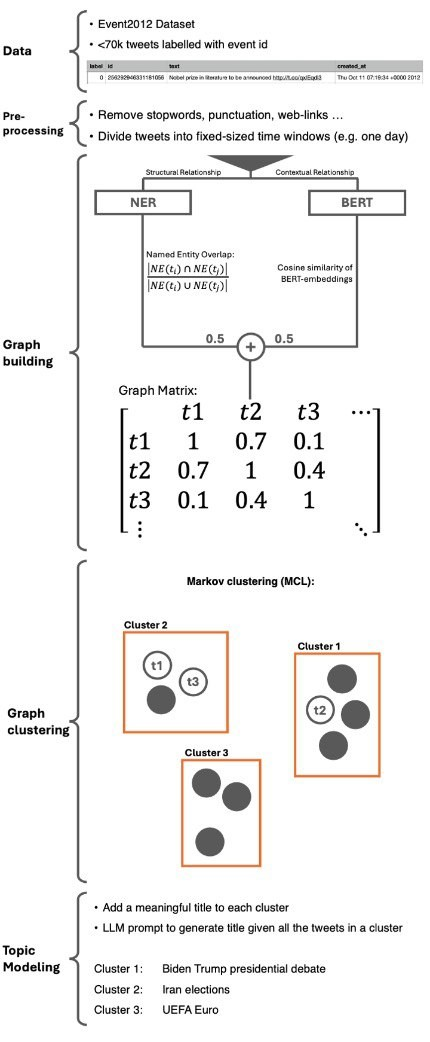
\includegraphics[width=0.95\linewidth]{Images/model.jpeg}
    \caption{Overview of the Social Media Monitoring Pipeline}
    \label{fig:model}
\end{figure}

As shown in Figure \ref{fig:model}, the process involves multiple stages including data preprocessing, graph building, and topic modeling.

\subsection{Preprocessing}
\label{sec:preprocessing}
The preprocessing stage is essential for cleaning and preparing tweets before further analysis. The process involves the following steps:
\begin{itemize}
\item Lowercasing: All tweets are converted to lowercase to ensure uniformity in text analysis.

\item Tokenization: Tweets are tokenized using the TweetTokenizer from the NLTK library\footnote{\url{https://www.nltk.org/}}, which is specifically designed to handle social media text.

\item Removing Short Tweets: Tweets with fewer than three words are discarded, as they are unlikely to provide meaningful information.

\item Stopword Removal: Common stopwords are removed from the tweets to focus on more informative words.

\item Web Links Removal: Web links starting with "http" or "www" are removed from the tweets, as they often add noise to the data.

\item Punctuation Removal: Punctuation marks are removed from tokens, except for hashtags, which are retained for their relevance in social media contexts.

\item Non-ASCII Characters Removal: Non-ASCII characters are removed to avoid encoding issues during further processing.

\item Retweet Removal: Retweets can be filtered out as needed, although this step is currently optional in the implementation.

\item Cleaning Empty Tokens: Any remaining empty tokens are removed to ensure clean data.
\end{itemize}
After normalization, only tweets that have been successfully processed and contain meaningful content are retained for further analysis. This preprocessing ensures that the data used in the subsequent stages is clean, consistent, and relevant for event detection.

\subsection{Graph Construction}
\label{sec:graphconstruction}
In the graph construction module, tweets are processed and modeled as a graph, where nodes represent tweets and edges represent the similarities between tweets. This similarity computation is crucial for clustering tweets related to specific events. In this study, we use the similarity metric proposed by \citet{edtbert} in the EDT\textsubscript{BERT} model, that is designed to capture both the structural associations and contextual relationships between tweets.

\subsubsection{Contextual Embeddings}
\label{sec:contextualembeddings}
In order to capture contextual knowledge, it is essential to convert textual input into vector representations, which can then be used to calculate the similarity between tweets. Various embedding techniques, such as One-Hot Encoding and Term Frequency Inverse Document Frequency (TFIDF), can be employed for this purpose. However, not all techniques are capable of adequately capturing the contextual nuances present in tweets. To address this, a pre-trained BERT sentence transformer \citep{sentence-bert} was utilized, specifically the all-mpnet-base-v2\footnote{\url{https://huggingface.co/sentence-transformers/all-mpnet-base-v2}} model, to encode the preprocessed tweets. Each tweet is passed through the BERT embedding module, resulting in a dense 768-dimensional vector. The contextual similarity between tweet vectors is then calculated using the cosine similarity measure. In the graph of tweets, each node represents a tweet as a 768-dimensional BERT embedding vector, and edges connect tweets if their semantic similarity exceeds a predefined threshold (in the experiment, the threshold is set to 0.29). The Structural Relation (SR) and Contextual Similarity (CS) are given equal weight in our approach, as done in the EDT\textsubscript{BERT} model.


\subsubsection{Structural Embeddings}
\label{sec:structuralembeddings}
To establish structural relationships, the graph construction also considers the overlap of hashtags and named entities (NEs) between tweets. These overlaps indicate the formation of cliques, where tweets are interconnected due to their association with common events. The degree of overlap in hashtags and named entities between two tweets is calculated using the Jaccard Similarity measure. This measure is used to quantify the structural similarity between tweets, with the structural relationship between two tweets being a combination of their hashtag overlap and named entity overlap.

\subsection{Graph Clustering}
\label{sec:graphclustering}
Using the structural relationship and contextual knowledge, a tweet graph is generated from preprocessed tweets. And the tweet graph is passed to the next module for the event detection task. In this study, the Markov clustering (MCL) method \cite{mcl} is used to analyze the graph representation of tweets, aiming to detect clusters of related tweets. The MCL algorithm has the capability to split the graph into clusters without requiring the number of clusters to be specified as an input parameter. The methodology employed in this technique is based on the idea that clusters are present inside a given graph. It utilizes a random walk approach to aid the process of clustering.



\subsection{Event Summarization}
\label{sec:eventsummarization}
The event summarization component of the Social Media Monitoring system is designed to generate concise and informative descriptions of detected event clusters on social media. This component combines traditional natural language processing (NLP) techniques with state-of-the-art large language models (LLMs) to produce meaningful summaries of event-related tweet clusters.

\subsubsection{Top Words Extraction} For each detected cluster, the most salient keywords that characterize the cluster are extracted. Tweets within each cluster are preprocessed and represented in a term-document matrix, allowing the identification of the most frequently occurring unigrams, bigrams, and trigrams. This process is facilitated using the CountVectorizer from the scikit-learn\footnote{\url{https://scikit-learn.org/stable/}} library. The extracted top words provide a preliminary summary of the cluster's content, highlighting the core topics being discussed.

\subsubsection{Cluster Summarization} To generate more comprehensive summaries, Google's FLAN-T5 \cite{google-flan-t5}, a transformer-based sequence-to-sequence model, is employed. The top words from each cluster serve as prompts for the model, which then generates a concise textual summary that encapsulates the primary themes of the cluster. This method ensures that the generated summaries are both coherent and contextually relevant, making them suitable for integration into automated news content generation. In this study, google/flan-t5-base\footnote{\url{https://huggingface.co/google/flan-t5-base}} model is used.

\subsubsection{Topic Detection} In addition to summarization, the overarching topic of each cluster is classified using a pre-trained topic classification model tailored for Twitter content. This model assigns clusters to predefined categories such as "arts \& culture," "business \& entrepreneurs," "pop culture," "daily life," "sports \& gaming" and "science \& technology." The classification is performed using a transformer-based model cardiffnlp/tweet-topic-latest-single\footnote{\url{https://huggingface.co/cardiffnlp/tweet-topic-latest-single}} developed by \citet{twitter-topic-classification}, which outputs the most likely topic based on the content of the tweets in each cluster. The distribution of topics across clusters is visualized using a pie chart, providing insights into the dominant themes in the detected events, as shown in the Figure \ref{fig:pie_chart}.

\begin{figure}[htbp]
    \centering
    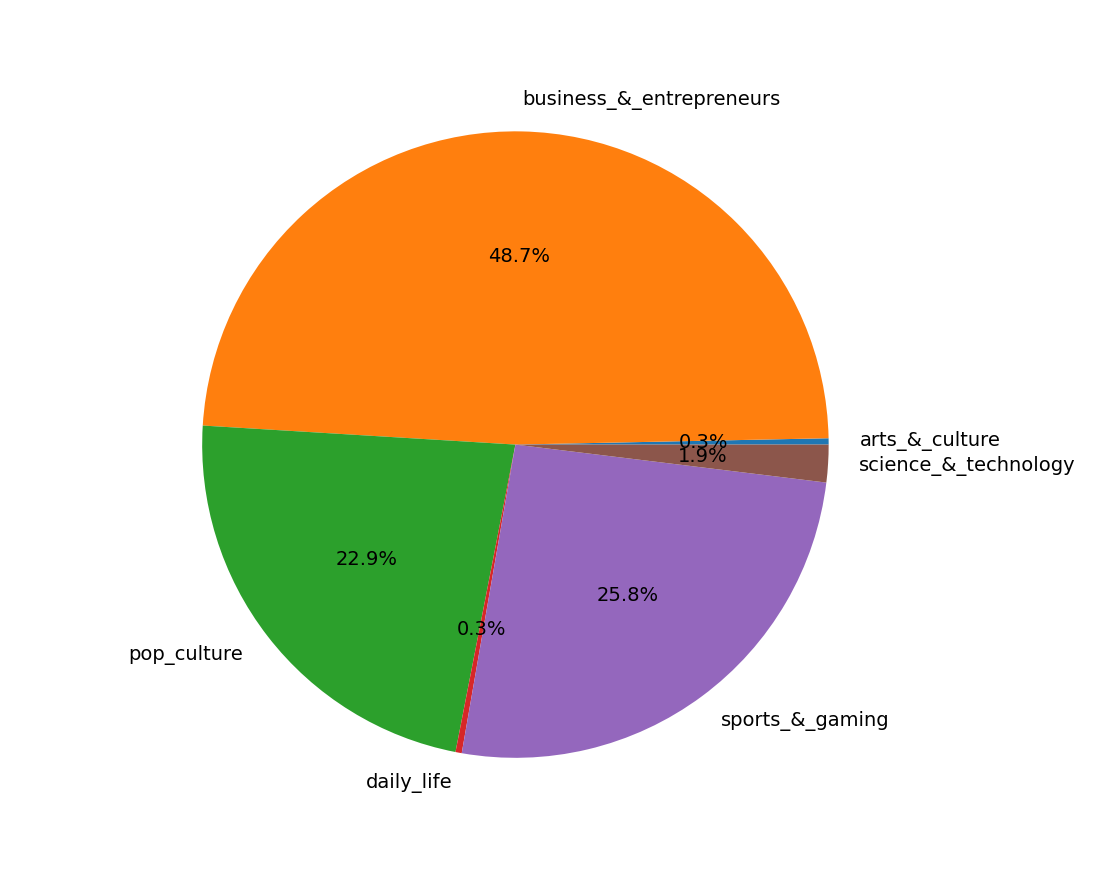
\includegraphics[width=1\linewidth]{Images/pie_chart.png}
    \caption{Distribution of Tweet Topics}
    \label{fig:pie_chart}
\end{figure}

\subsubsection{Output} The final output of the event summarization module includes a detailed summary for each cluster, a list of the most relevant keywords, the identified topic, and the size of the cluster. This output is crucial for understanding the context and significance of the detected events. 

By integrating advanced NLP techniques with LLMs, the event summarization component enhances the automated detection and reporting of social media events, contributing to the overall goal of producing high-quality, automated news content.

\subsection{Dashboard Implementation} 
\label{sec:dashboard}
The Event Monitoring Dashboard provides a visual interface for users to explore detected events and their relevance. Implemented using Streamlit\footnote{\url{https://streamlit.io/}}, the dashboard enables users to visualize the clustering results, facilitating a better understanding of how events are grouped based on structural and contextual similarities, as shown in the Figure \ref{fig:dashboard}.

\begin{figure}[htbp]
    \centering
    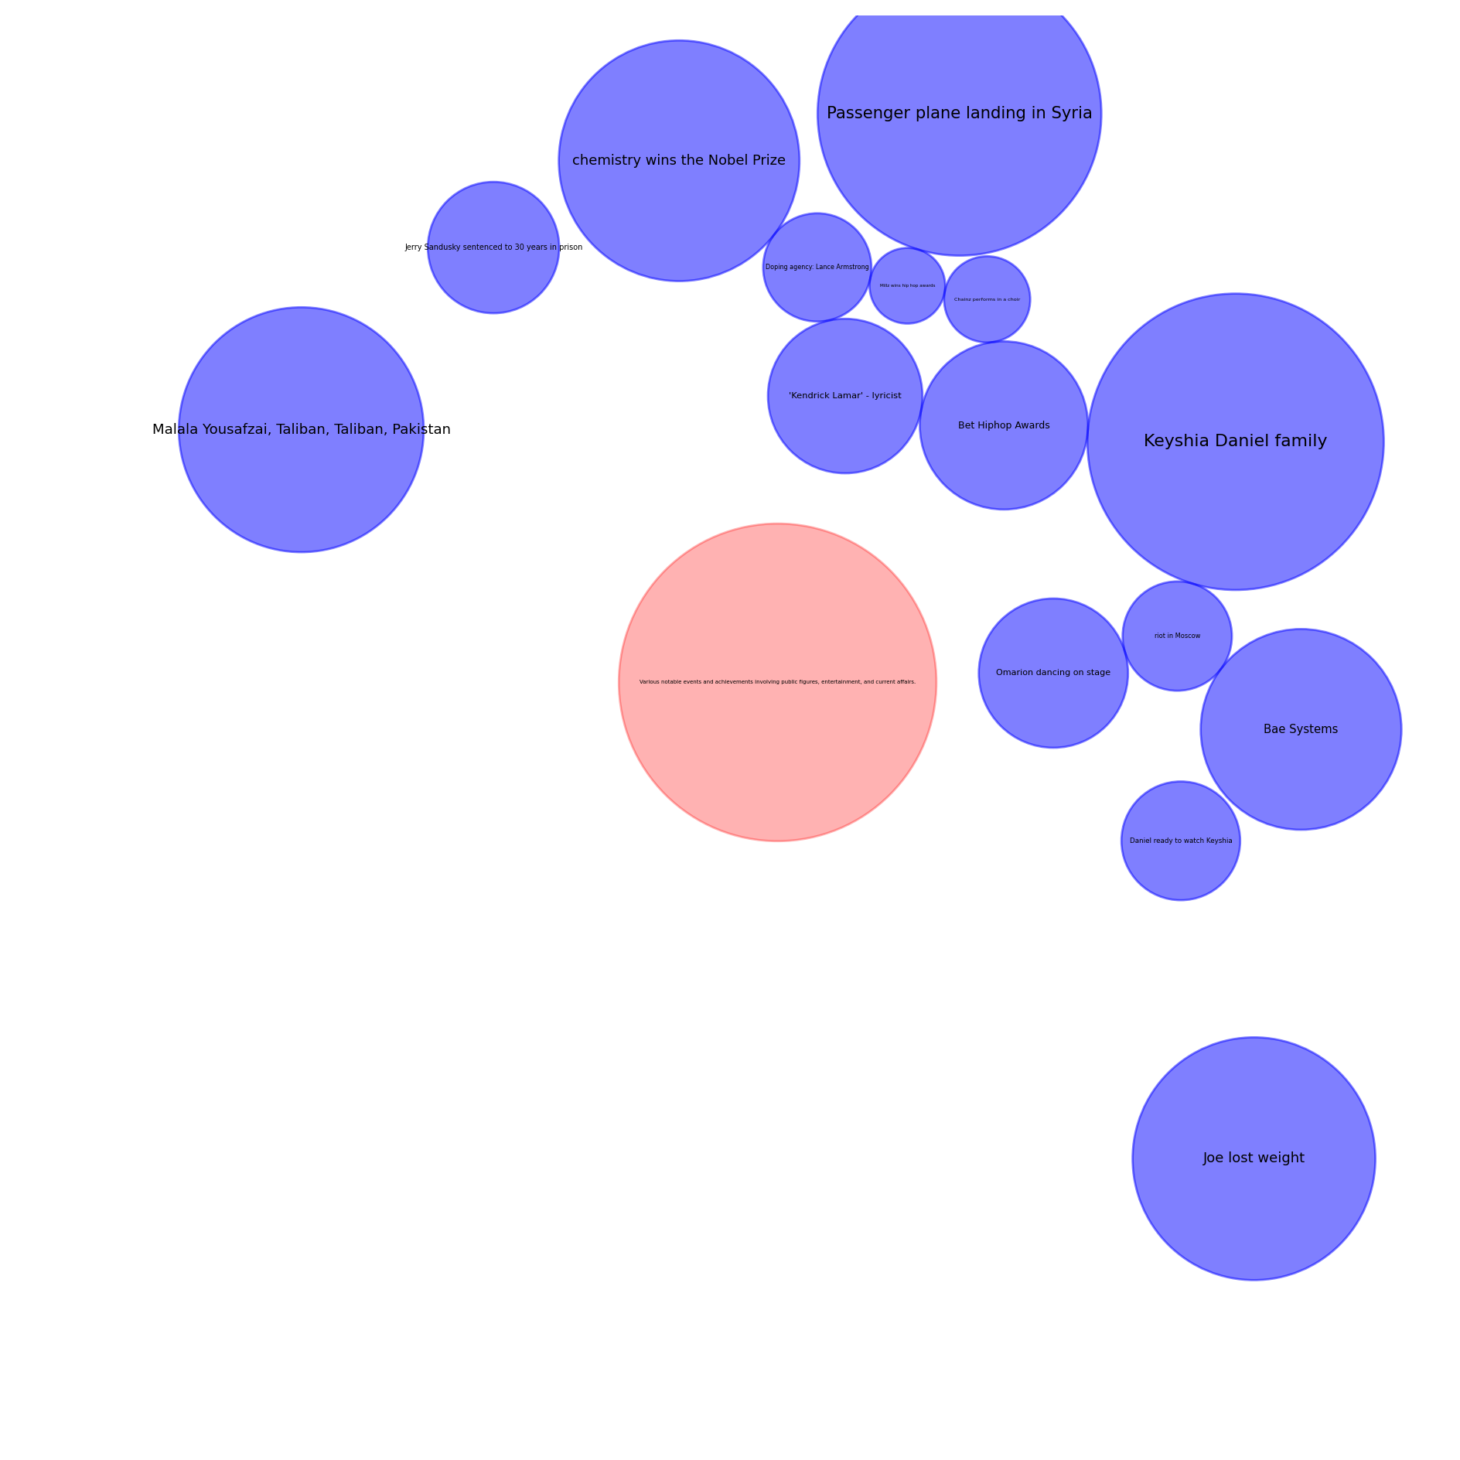
\includegraphics[width=1\linewidth]{Images/dashboard.png}
    \caption{Visualization of the Clusters}
    \label{fig:dashboard}
\end{figure}
\subsubsection{Data Preparation} 
The dashboard begins by setting up the page layout to be wide, ensuring that the visualization can utilize the full screen space available. The key input to this dashboard is a preprocessed dataset containing tweet summaries, which is loaded from a JSON file. This dataset is converted into a pandas DataFrame for ease of manipulation and display.

\subsubsection{Event Representation and Similarity Calculation}  

To identify the relevance of events, the dashboard employs vectorization techniques. Using the Sent2Vec\footnote{\url{https://pypi.org/project/sent2vec/}} vectorizer, each tweet summary, along with a predefined query, is converted into vector embeddings. These vectors are used to compute the cosine similarity between the query and each tweet summary, allowing us to measure how closely each summary aligns with the topic of interest.

\subsubsection{Visualization: Mapping Similarity to a 2D Plane}   

The dashboard visualizes the similarity between events by mapping these values onto a 2D plane. This is achieved by normalizing the similarity scores and then using trigonometric functions (cosine and sine) to generate coordinates for each event. The resulting 2D coordinates are scaled to fit within a defined range, ensuring that all events are visually distinguishable.

\subsubsection {Radius Calculation and Overlap Resolution}

Each event is represented as a circle, with the radius corresponding to the size of the event cluster. Larger clusters are depicted with larger circles, signifying their importance. To avoid overlapping circles, an iterative algorithm is implemented to adjust the positions of circles that overlap, ensuring a clear and uncluttered visualization.

\subsubsection {Plotting and Display}

The dashboard then draws these circles on a matplotlib plot, annotating each with the event summary. A central circle represents the query topic, serving as a reference point for the related events. The plot is carefully configured to maintain aspect ratio and avoid distortion, and the axes are turned off to emphasize the event clusters visually.


\subsection{Integration to the Automated Journalist App}
\label{sec:integration}
The integration of the event detection functionality into the existing Automated Journalist App aims to enhance its capabilities by identifying significant events from social media posts retrieved by a user query. The primary objective is to detect these events and visualize them using the developed dashboard. For this purpose, an Event Detection Module has been constructed, consisting of a Flask\footnote{\url{https://flask.palletsprojects.com/en/3.0.x/}} Backend and a Streamlit Frontend. Both must be run in parallel with the Automated Journalist App. The Flask Backend offers two API endpoints: "update-events", which receives social media posts from the automated journalist app to execute the event detection process, and "/events", which returns the list of current events detected. The Streamlit Frontend proactively requests the current events from the "/events" endpoint every five seconds to ensure that the dashboard remains up-to-date with the latest information. To facilitate this integration seamlessly, a "Detect Events" button has been added to the feed of the Automated Journalist App. When clicked, the button sends the current feed to the event detection backend, triggering the event detection process, and subsequently, the Streamlit Frontend presents the updated dashboard to the user, showcasing the detected events in real-time. A screenshot from the Automated Journalist App is shown in the Figure \ref{fig:integration}.

\begin{figure}[htbp]
    \centering
    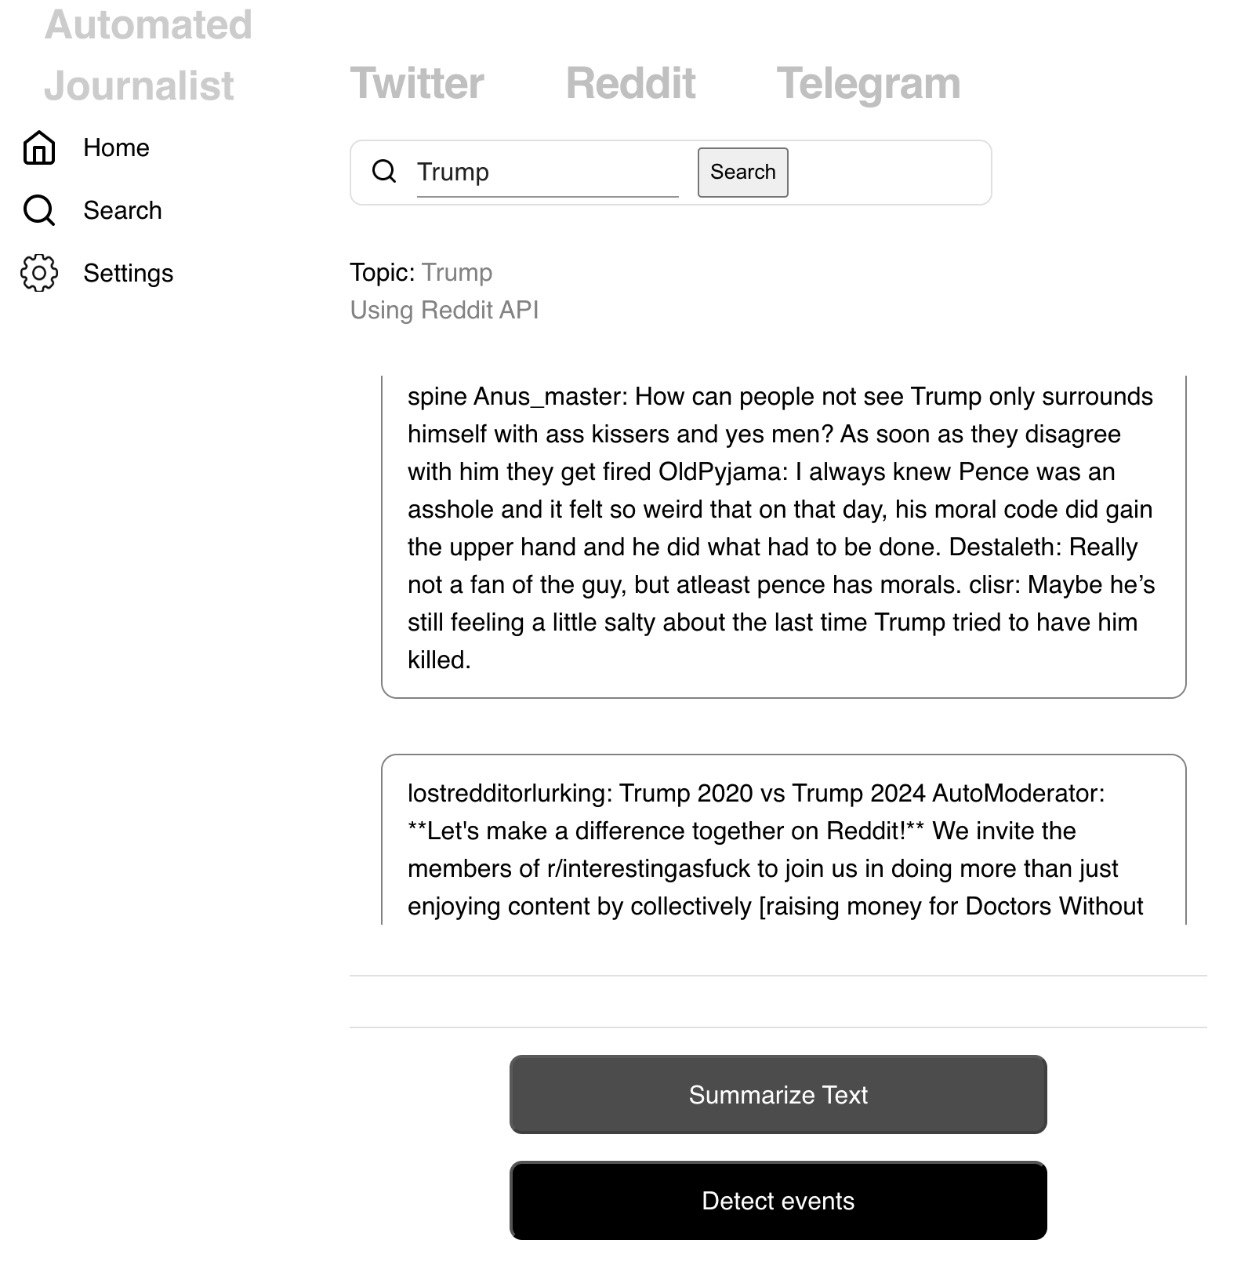
\includegraphics[width=0.95\linewidth]{Images/integration.jpeg}
    \caption{Social Media Monitoring module integrated into the Automated Journalist App}
    \label{fig:integration}
\end{figure}